\documentclass[]{scrartcl}
\usepackage{graphicx}
\usepackage{geometry}
\geometry{
	a4paper,
	total={170mm,257mm},
	left=20mm,
	top=20mm,
}


%opening
\title{Software Design Description}
\author{Brandon Smith, Nieka Gutenberger, Joseph Coppin, Ryan Frazier, Trevor Jewkes}

\begin{document}

\maketitle
\section{Software Design}
\subsection{Login Screen}

\centerline{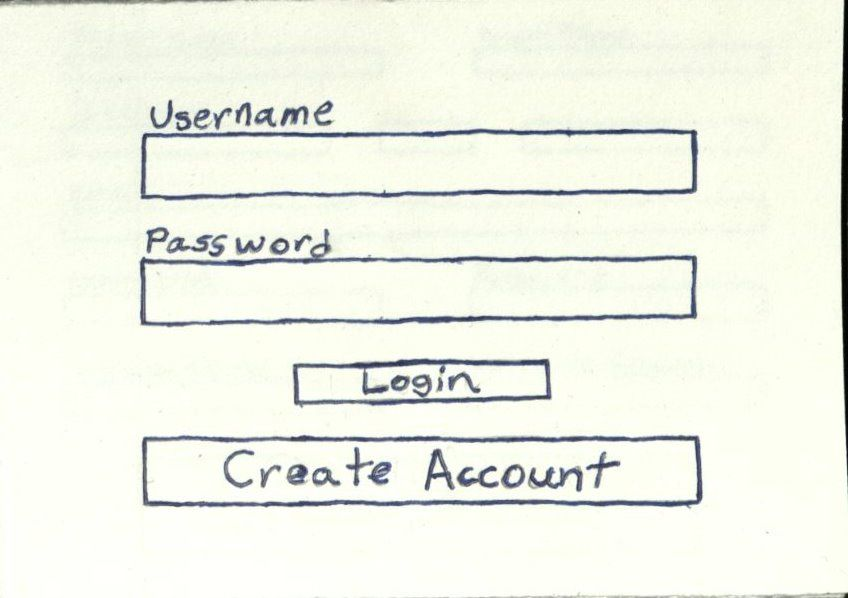
\includegraphics{1.jpg}}

This screen is the first screen the user will see.  It has a text box for the user to enter a user name and password.  It also has two buttons a “login” which sends the username and password to the server, and brings up Screen 3; and a “Create Account” button which takes the user to Screen 2. where they can create their account prior to playing games. 

\subsection{Account Creation}
%Figure 2%
\centerline{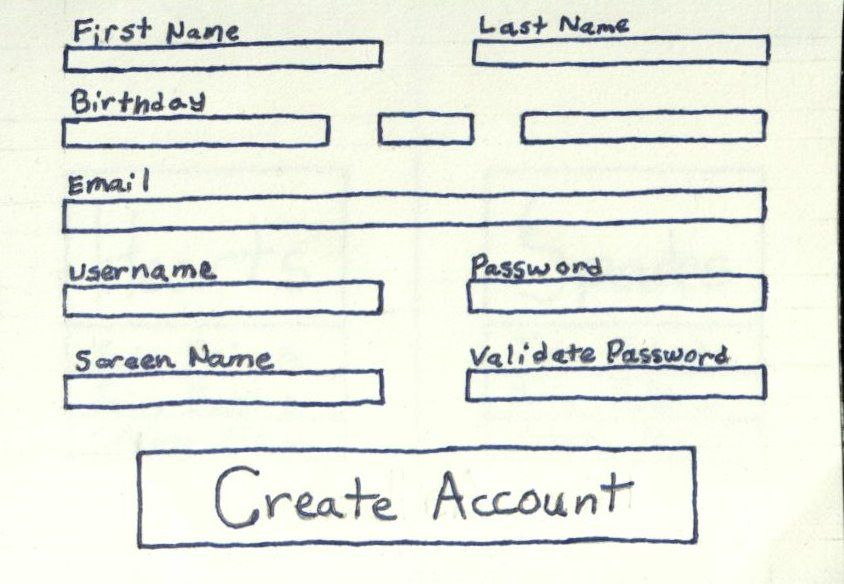
\includegraphics{2.jpg}}
This screen is the screen that appears after the User clicks the “Create Account” Button.  It has text fields for all the information needed to create an account including Name, “First” and “Last”, “Birthday”, “E-mail”, “Username”, “Password” “Screen Name” and “Verify Password”,  Finally the page includes a “Create Account” button which sends all information to the server so it can create the account.  

\subsection{Main Menu}
\centerline{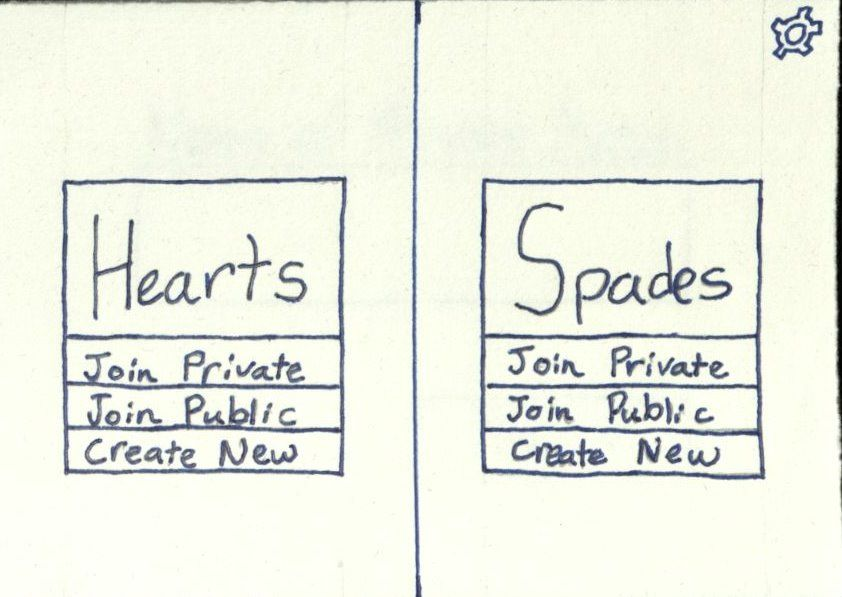
\includegraphics{3.jpg}}
This screen is the main menu for the Game, it is divided in half with one half related to the game of Hearts, and the other half for the game of Spades.  Each half includes three buttons, “Join Private”, “Join Public” and “Create New”.  The “Join Private” brings up Screen 4, which allows the user enter the name of the game they want to join.  The “Join Public” will tell the server to assign the user to the first available  public game, if no game is available the server will create a new game with the user and three AI players.  Finally the “Create New” button will bring up Screen 5. which asks for the users preferences to create a new game.

\subsection{Join Private}
\centerline{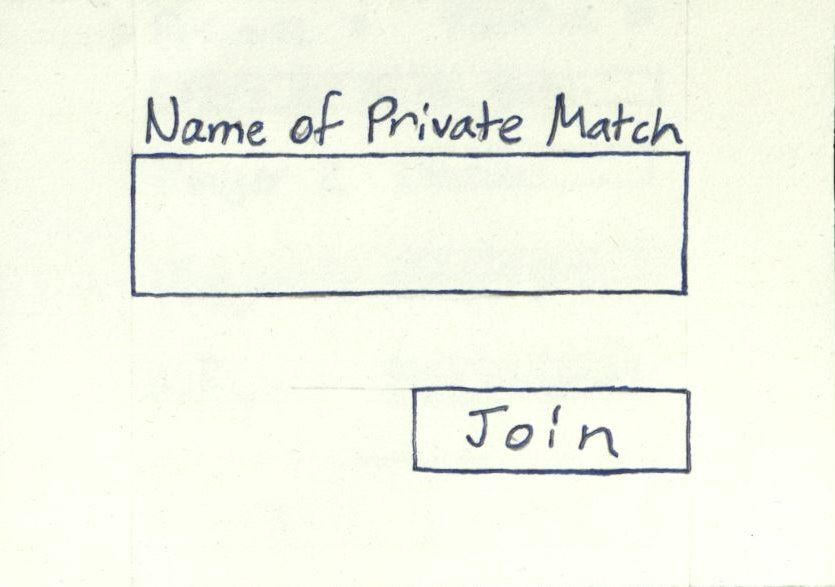
\includegraphics{4.jpg}}
This Screen appears when a user has selected to Join a Private game it is very simple it includes a a text box for the user to enter the name of the game they wish to join. 

\subsection{Create New}
\centerline{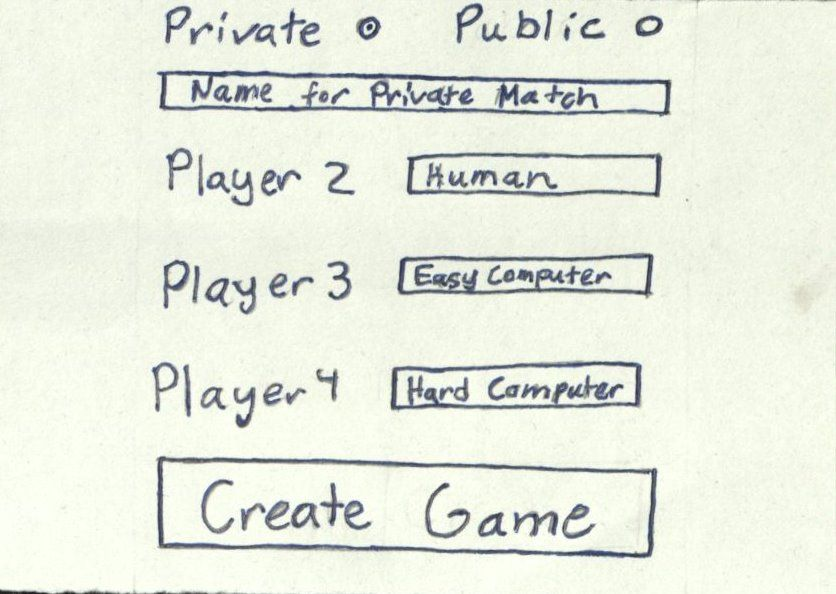
\includegraphics{5.jpg}}
This Screen appears when a user requests to create a new game it includes a radio button to select either a public or private game.  If private is selected a text box is activated for the user to enter a name for the game.  Next is a set of radio buttons allowing the user to select 1, 2, or 3 additional human players.  Next the user selects the lever of the AI, and finally a “Create Game” Button which sends the information to the server and creates the new game.  

\subsection{Place Bid}
\centerline{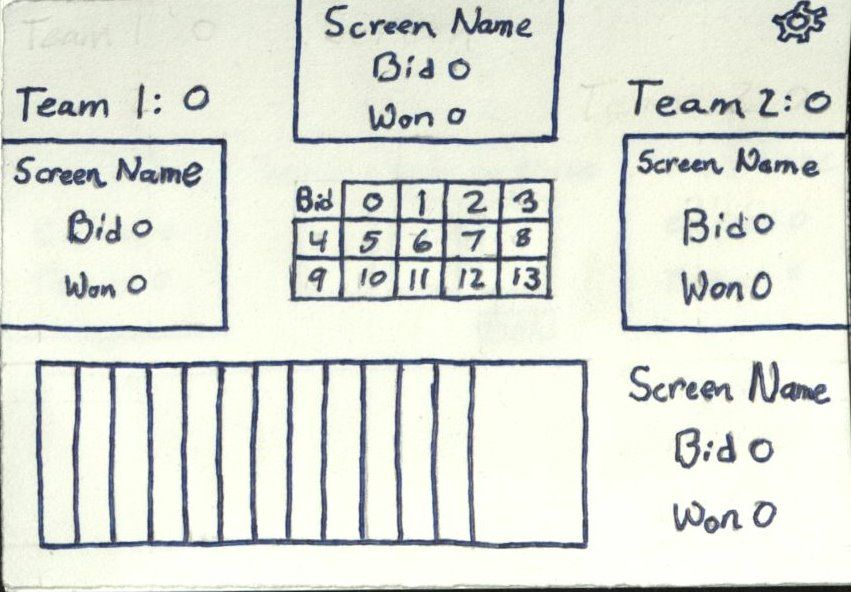
\includegraphics{6.jpg}}
This view will prompt the user to place a bid while playing the game of Spades. They will choose a bid from the ones provided.

\subsection{Pass Cards}
\centerline{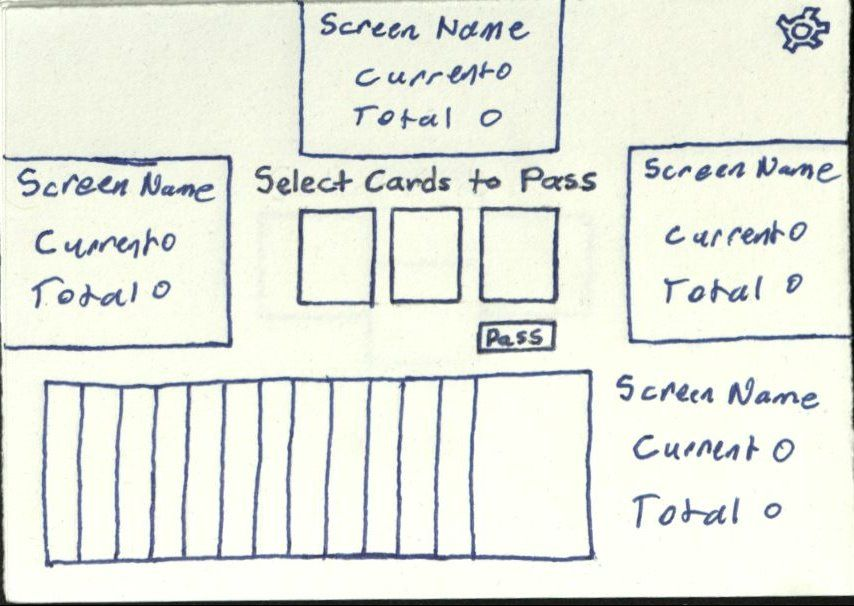
\includegraphics{7.jpg}}
This view will prompt the user to choose 3 of their cards which they will pass while playing the game of Hearts. Once the cards have been chosen, the "Pass Cards" button will need to be pressed to move on.

\subsection{Game Play}
\centerline{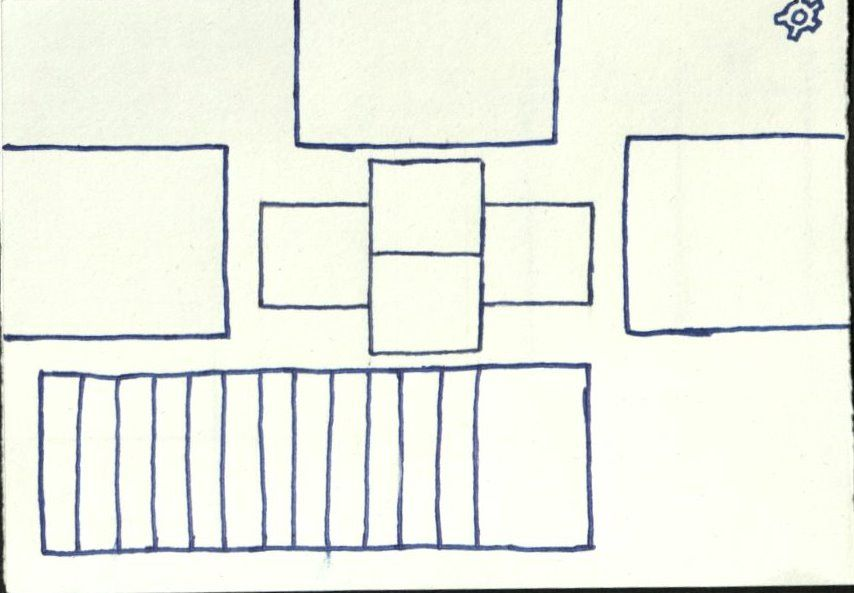
\includegraphics{8.jpg}}
This screen will be the view that will be use for play of the game. Since Spades and Hearts have the same basic set-up we can use the same view for both. It shows the players hand along with the scores of the other players.

\subsection{Scoreboard}
\centerline{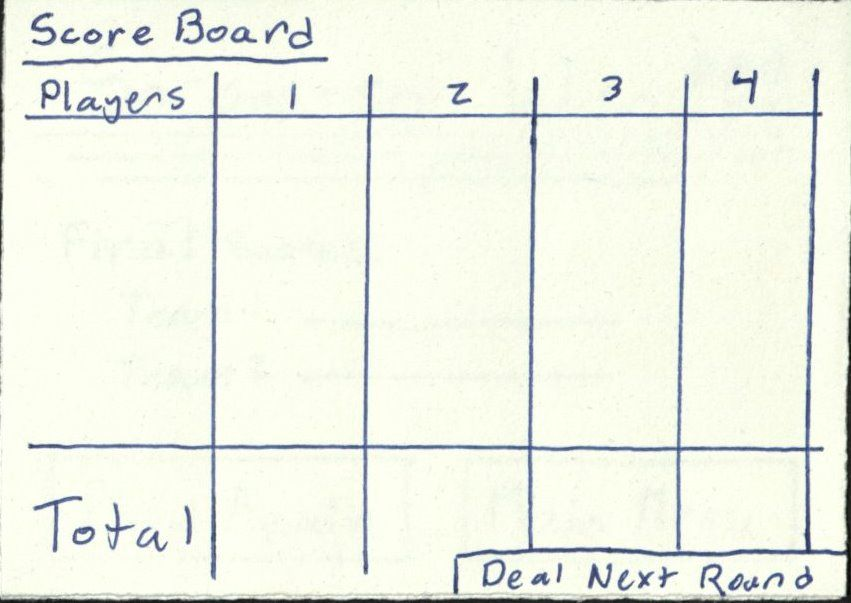
\includegraphics{9.jpg}}
This is the scoreboard that will be shown inbetween rounds. It will show the scores for all the following rounds. There is a "Deal" button that will be use to move to the next round.

\subsection{End-of-Game}
\centerline{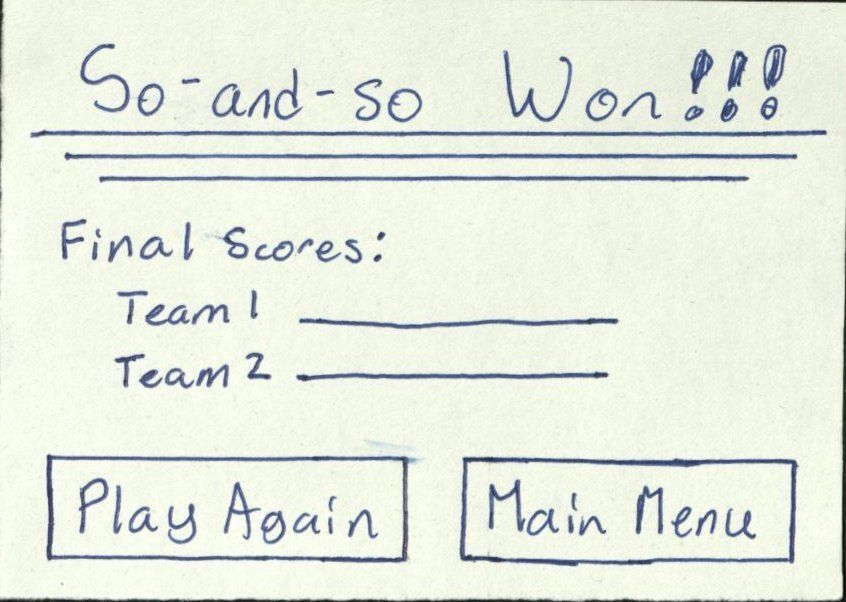
\includegraphics{10.jpg}}
This the End-of-Game screen. It will display the winner of the game along with the final scores for the game. There are two buttons, "Play Again" and "Main Menu". The "Play Again" button is used to play again with the same players. The "Main Menu" button will return the user to the main menu.
\end{document}
